\documentclass[a4paper,11pt]{article}

%Headers
\usepackage[dvips]{graphicx}    %package that does pdfs
\usepackage{color}              %this needs to be here also
\usepackage{ulem}
\usepackage{amsmath}
\usepackage{pgfplots}
\usepackage{adjustbox}
\usepackage{graphicx}
\usepackage{enumitem}


\newcommand{\mybf}[1]{\boldsymbol{#1}}
\newcommand{\norm}[1]{\lvert\lvert #1 \rvert\rvert}

\title{%
	Problem Set 1\\
	\large MIT CW Linear Algebra (18.06)
}
\author{Aviel Livay}
\date{\today}

\begin{document}
\maketitle


\section*{Section 1.1}
\subsection*{Problem 23}
If we look at all combinations of $\mybf{u}$, $\mybf{v}$ and $\mybf{w}$ then there's no vector that can't be produced from $c\mybf{u}+d\mybf{v}+e\mybf{w}$. If however $\mybf{u}$, $\mybf{v}$ and $\mybf{w}$ are on the same plane then there are many vectors that can't be produced - all vectors that are outside that plane.

\subsection*{Problem 28}

We know that 
\begin{equation}
       \mybf{v}+\mybf{w} = (4,5,6)\label{eq:1}
\end{equation}
\begin{equation}
       \mybf{v}-\mybf{w} = (2,5,8)\label{eq:2}
\end{equation}

adding $\eqref{eq:1}+\eqref{eq:2}$ we get

\begin{subequations}

\begin{align}
    2.\cdot\mybf{v} &= (6,10,14)\label{eq:2v}\\
    \mybf{v} &= (3,5,7)\label{eq:v}
\end{align}
\end{subequations}

subtructing $\eqref{eq:1}-\eqref{eq:2}$ we get

\begin{subequations}
\begin{align}
    2.\cdot\mybf{w} &= (2,0,-2)\label{eq:2w}\\
    \mybf{w} &= (1,0,-1)\label{eq:w}
\end{align}
\end{subequations}


This is a question with two 2 unknown numbers, and an equal number of equations to find those numbers.

\section*{Section 1.2}
\subsection*{Problem 23}
The figure shows that $\cos\alpha = v_1/\norm{v}$ and $\sin\alpha = v_2/\norm{v}$. Similarly $\cos\beta = w_1/\norm{w}$ and $\sin\beta = w_2/\norm{w}$

\begin{subequations}
\label{eq:optim}
\begin{align}
    &\cos(\beta-\alpha)\\
    =& \cos\beta\cdot\cos\alpha + \sin\beta\cdot\sin\alpha\\
    =& v_1/\norm{\mybf{v}} \cdot w_1/\norm{\mybf{w}} + w_2/\norm{\mybf{w}} \cdot v_2/\norm{\mybf{v}}\\
    =& \frac{v_1 \cdot w_1 + v_2 \cdot w_2}{\norm{\mybf{v}} \cdot \norm{\mybf{w}}}\\
    =& \frac{\mybf{v} \cdot \mybf{w}}{\norm{\mybf{v}} \cdot \norm{\mybf{w}}}
\end{align}
\end{subequations}

\subsection*{Problem 28}
All $x$ and $y$ combinations that meet $x+2y=5$ are located on the linear line $y=-0.5x+2.5$.\\

\begin{adjustbox}{center}
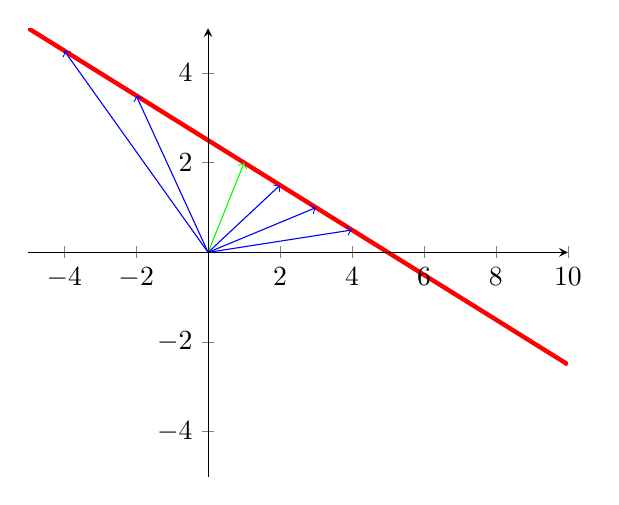
\begin{tikzpicture}
\begin{axis}[
    xmin=-5, xmax=10,
    ymin=-5, ymax=5,
    axis lines=center,
    axis on top=true,
    domain=-5:10,
    ]
    \addplot [mark=none,draw=red,ultra thick] {-0.5*x+2.5};
    after end axis/.code={
               \draw[green,->] (axis cs:0,0) -- (axis cs:1,2);
               \draw[blue,->] (axis cs:0,0) -- (axis cs:2,1.5);
               \draw[blue,->] (axis cs:0,0) -- (axis cs:3,1);
               \draw[blue,->] (axis cs:0,0) -- (axis cs:4,0.5);   
               \draw[blue,->] (axis cs:0,0) -- (axis cs:-2,3.5); 
               \draw[blue,->] (axis cs:0,0) -- (axis cs:-4,4.5);        
               }]
\end{axis}
\end{tikzpicture}
\end{adjustbox}

The shortest distance to the line $y=-0.5x+0.5$ has to have a slope of 2, so the line that starts in the center is $y=2x$ so the shortest $\mybf{w}$ is $(1,2)$. Also we know that
\begin{equation}
       cos(\beta-\alpha) = \frac{\mybf{v}\cdot\mybf{w}}{\norm{\mybf{v}}\cdot\norm{\mybf{w}}}\\
\end{equation}

given that both $\mybf{v}\cdot\mybf{w}$ and $\norm{\mybf{v}}$ are constants then finding the shortest $\mybf{w}$

\begin{equation}
	   \min_{\substack{\mybf{w}}}\norm{\mybf{w}} = \frac{\mybf{v}\cdot\mybf{w}}{\norm{\mybf{v}}\cdot\cos(\beta-\alpha)}\\
\end {equation}

is actually finding the maximum here:
\begin{equation}
\max_{\substack{\mybf{w}}}{\cos(\beta-\alpha)}
\end {equation}

which happens when $\beta$ = $\alpha$, which means both $\mybf{v}$ and $\mybf{w}$ are on the same line.

\section*{Section 1.3}
\subsection*{Problem 4}

  \begin{align}
    y &= x1\cdot\mybf{w1}+x2\cdot\mybf{w2}+x3\cdot\mybf{w3} \\
    &=
    	x1
    	\begin{bmatrix}
           1 \\
           2 \\
           3
         \end{bmatrix}
         + 
    	x2
    	\begin{bmatrix}
           4 \\
           5 \\
           6
         \end{bmatrix}
                  + 
    	x3
    	\begin{bmatrix}
           7 \\
           8 \\
           9
         \end{bmatrix}
         =
        \begin{bmatrix}
           0 \\
           0 \\
           0
         \end{bmatrix}
  \end{align}
  
  It's easy to see that $\mybf{w1}=2\mybf{w2}-\mybf{w3}$ which means that they are dependent and it's thus possible to have $\mybf{w1}-2\mybf{w2}+\mybf{w3}=\mybf{0}$. The three vectors thus lie in a plane and the matrix $\mybf{W}$ with those three columns is not invertible.
  
\subsection*{Problem 13}
Here's the equation:
\begin{align}
\begin{bmatrix}
0  & 1  & 0  & 0  & 0 \\
-1 & 0  & 1  & 0  & 0 \\
0  & -1 & 0  & 1  & 0 \\
0  & 0  & -1 & 0  & 1 \\
0  & 0  & 0  & -1 & 0 
\end{bmatrix}
\cdot
\begin{bmatrix}
x1  \\
x2 \\
x3 \\
x4 \\
x5 
\end{bmatrix}
=
\begin{bmatrix}
b1  \\
b2 \\
b3 \\
b4 \\
b5 
\end{bmatrix}
\end{align}

Writing up the equations in order to get 0:
\begin{align}
\begin{bmatrix}
x2 \\
-x1+x3 \\
-x2+x4 \\
-x3+x5 \\
-x4 
\end{bmatrix}
=
\begin{bmatrix}
0  \\
0 \\
0 \\
0 \\
0 
\end{bmatrix}
\end{align}
Immediately we can see that both $x2$ and $x4$ must equal 0 and replacing them yields:

\begin{align}
\begin{bmatrix}
0 \\
-x1+x3 \\
0 \\
-x3+x5 \\
0
\end{bmatrix}
=
\begin{bmatrix}
0  \\
0 \\
0 \\
0 \\
0 
\end{bmatrix}
\end{align}

And then if we say that $x1=x3=x5=C$ then we end up with $\mybf{x}=(C, 0, C, 0, C)$ as the solution for every $C$.

$C\mybf{x}=b$ can be solved only if $b1+b3+b5=0$. Each column of $C$ is in this plane. 

\section*{Section 2.1}
\subsection*{Problem 29}

\begin{subequations}
\begin{align}
\mybf{u_1}&=
\begin{bmatrix}
0.8 & 0.3\\
0.2 & 0.7
\end{bmatrix}
\cdot
\begin{bmatrix}
1  \\
0 
\end{bmatrix}
=
\begin{bmatrix}
0.8  \\
0.2 
\end{bmatrix}
+
\begin{bmatrix}
0  \\
0 
\end{bmatrix}
=
\begin{bmatrix}
0.8  \\
0.2 
\end{bmatrix}
\\
\mybf{u_2}&=
\begin{bmatrix}
0.8 & 0.3\\
0.2 & 0.7
\end{bmatrix}
\cdot
\begin{bmatrix}
0.8  \\
0.2 
\end{bmatrix}
=
\begin{bmatrix}
0.64  \\
0.16 
\end{bmatrix}
+
\begin{bmatrix}
0.06  \\
0.14 
\end{bmatrix}
=
\begin{bmatrix}
0.7  \\
0.3 
\end{bmatrix}
\\
\mybf{u_3}&=
\begin{bmatrix}
0.8 & 0.3\\
0.2 & 0.7
\end{bmatrix}
\cdot
\begin{bmatrix}
0.7  \\
0.3 
\end{bmatrix}
=
\begin{bmatrix}
0.56  \\
0.14 
\end{bmatrix}
+\begin{bmatrix}
0.09  \\
0.21 
\end{bmatrix}
=
\begin{bmatrix}
0.65  \\
0.35 
\end{bmatrix}
\\
\mybf{u_4}&=
\begin{bmatrix}
0.8 & 0.3\\
0.2 & 0.7
\end{bmatrix}
\cdot
\begin{bmatrix}
0.65  \\
0.35 
\end{bmatrix}
=
\begin{bmatrix}
0.52  \\
0.13 
\end{bmatrix}
+\begin{bmatrix}
0.105  \\
0.245 
\end{bmatrix}
=
\begin{bmatrix}
0.625  \\
0.375 
\end{bmatrix}
\end{align}
\end{subequations}

I notice the the sum of the vector elements stays 1.\\
Proof by induction:\\
The sum of elements in $\mybf{u_0}$ is 1.\\
Suppose that the sum of elements in $\mybf{u_n}$ is 1. 
We also know that the sum of the elements in each of $\mybf{A}$ columns is 1.
\begin{align}
\mybf{u_1}&=
\begin{bmatrix}
a_{1,1} & a_{1,2}\\
a_{2,1} & a_{2,2}
\end{bmatrix}
\cdot
\begin{bmatrix}
u^n_1  \\
u^n_2 
\end{bmatrix}
=
u^n_1
\cdot
\begin{bmatrix}
a_{1,1}  \\
a_{2,1}
\end{bmatrix}
+
u^n_2
\cdot
\begin{bmatrix}
a_{1,2}  \\
a_{2,2} 
\end{bmatrix}
=
\begin{bmatrix}
u^{n+1}_1  \\
u^{n+1}_2
\end{bmatrix}
\end{align}

\begin{align}
u^n_1 * (a_{1,1} + a_{2,1}) + u^n_2 * (a_{1,2} + a_{2,2})= u^n_1 + u^n_2 = 1 = u^{n+1}_1 + u^{n+1}_2 
\end{align}

\subsection*{Problem 30}



\begin{figure}[htbp]
\centerline{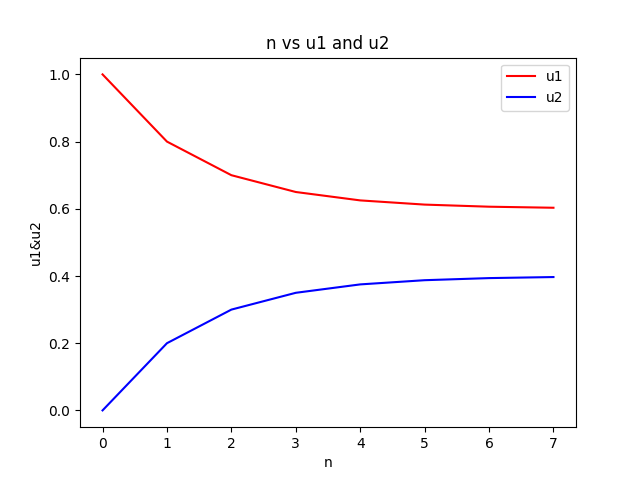
\includegraphics[scale=.5]{python/section_3_1_exercise_30_figure_1.png}}
\caption{Starting with u0 = (1,0).}
\label{fig:u_1_0}
\end{figure}

Figure~\ref{fig:u_1_0} illustrates the $(u^n_1, u^n_2)$ for $n$ running between 0 and 7 and where $(u^0_1, u^0_2) = (1,0)$\\

\begin{figure}[htbp]
\centerline{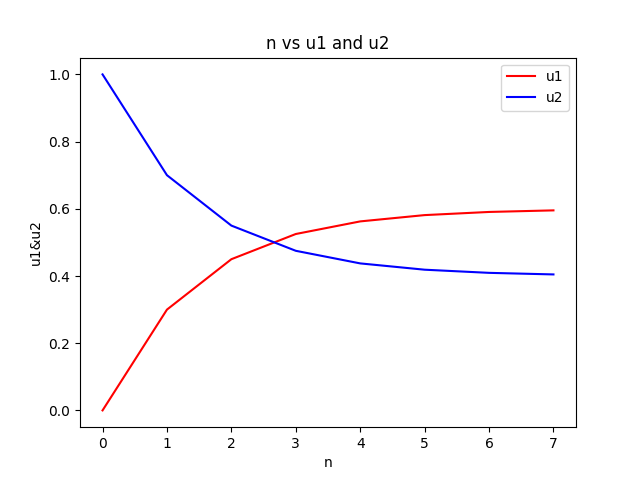
\includegraphics[scale=.5]{python/section_3_1_exercise_30_figure_2.png}}
\caption{Starting with u0 = (0,1).}
\label{fig:u_0_1}
\end{figure}
Figure~\ref{fig:u_0_1} illustrates the $(u^n_1, u^n_2)$ for $n$ running between 0 and 7 and where $(u^0_1, u^0_2) = (0,1)$\\

At the steady state:

\begin{align}
\begin{bmatrix}
0.8 & 0.3\\
0.2 & 0.7
\end{bmatrix}
\cdot
\begin{bmatrix}
x  \\
1-x 
\end{bmatrix}
=
\begin{bmatrix}
x  \\
1-x 
\end{bmatrix}
\end{align}
dot product of the first row gives:
\begin{align}
0.8x+0.3(1-x)=x
x=0.6
\end{align}
dot product of the second row confirms:
\begin{align}
0.2x+0.7(1-x)=1-x
x=0.6
\end{align}
so $\lim_{n \to \infty} u_n = (0.6,0.4)$

\section*{Section 2.2}
\subsection*{Problem 20}
Three planes can fail to have an intersection point, even if no planes are parallel.
The system is singular if row 3 of A is a linear combination of the first two rows. A third
equation that can't be solved together with $x + y + z = 0$ and $x - 2y - z = l$ if for example a row that adds the first row to twice the second row: $3x - 3y - z = 2$

\subsection*{Problem 32}
\begin{enumerate}[label=\alph*]
\item Elimination takes linear combinations of the rows. So this singular system has
the singular property: Some linear combination of the 100 rows is $0$.
\item Singular systems $\mybf{Ax} = \mybf{0}$ have infinitely many solutions. This means that some
linear combination of the 100 columns is $\mybf{0}$. 
\item an example of a 100 by 100 singular matrix with no zero entries would be
\begin{align}
\begin{bmatrix} 
    1 & 1 & \dots & 1\\
    1 & 1 & \dots & 2\\
    \vdots & \ddots & \\
    1 & 1 & \dots & 99\\
    2 & 2 & \dots & 100 
\end{bmatrix}
\end{align}
The last row is an addition of the first and second row.
\item first of all let's think about 3-dimensions
\begin{align}
\begin{bmatrix} 
    1 & 2 & 3\\
    2 & 3 & 4\\
    3 & 5 & 7 
\end{bmatrix}
\cdot
\mybf{x}
=
\begin{bmatrix} 
    0\\
    0\\
    0 
\end{bmatrix}
\end{align}
using elimination we get to
\begin{align}
\begin{bmatrix} 
    1 & 2 & 3\\
    0 & -1 & -2\\
    3 & 5 & 7 
\end{bmatrix}
\cdot
\mybf{x}
=
\begin{bmatrix} 
    0\\
    0\\
    0 
\end{bmatrix}
\end{align}
and
\begin{align}
\begin{bmatrix} 
    1 & 2 & 3\\
    0 & -1 & -2\\
    0 & -1 & -2 
\end{bmatrix}
\cdot
\mybf{x}
=
\begin{bmatrix} 
    0\\
    0\\
    0 
\end{bmatrix}
\end{align}
and
\begin{align}
\begin{bmatrix} 
    1 & 2 & 3\\
    0 & -1 & -2\\
    0 & 0 & 0 
\end{bmatrix}
\cdot
\mybf{x}
=
\begin{bmatrix} 
    0\\
    0\\
    0 
\end{bmatrix}
\end{align}
a possible solution would be $y=2$ and $z=1$. \\
which leads to $x=-7$ and $(-7, 2, 1)$.
so there's a non trivial linear combination of the columns that gives the vector $\mybf{0}$. \\\\
so back to our 100x100 matrix.\\\\
The row view states that there are 100 planes, all crossing the 0 point. The 2nd plane intersects with the first plan in 99 dimensions; The 3rd plane intersects with the first and second planes in 98 dimensions, etc. Overall 100 planes intersect not in one point as is with invertible matrices but with one line in 100 dimensions space. The missing rank. Therefore, there are an infinity of solutions along that line.\\\\
The column view states that there's an infinite number of linear combinations over the columns, that lead to the $\mybf{0}$ vector.
\end{enumerate}

\section*{Section 2.3}
\subsection*{Problem 22}
\begin{enumerate}[label=\alph*]
\item The third component of $\mybf{Ax}$ is $\sum a_{3,j}x_j = a_{3,1}x_1+a_{3,2}x_2+\dots+a_{3,n}x_n$
\item $\mybf{E_{2,1}A}_{2,1}$ = 0 because $\mybf{x_1}$ is eliminated from the second row during elimination.
\item In order to get rid of element $(2,1)$ we have to subtract $a_{2,1}/a_{1,1}$ from this element. So if we perform twice the same operation then the new $a_{2,1}$ is $-a_{2,1}/a_{1,1}$
\item The first component of $E_{21}A\mybf{x}$ is $\sum a_{1,j}x_j = a_{1,1}x_1+a_{1,2}x_2+\dots+a_{1,n}x_n$
\end{enumerate}

\subsection*{Problem 29}
(4) $\leftarrow$ (4) - (3)\\
\begin{align}
\begin{bmatrix} 
    1 & 0 & 0 & 0\\
    0 & 1 & 0 & 0\\
    0 & 0 & 1 & 0\\
    0 & 0 & \textcircled{-1} & 1\\ 
\end{bmatrix}
\cdot
\begin{bmatrix} 
    1 & 0 & 0 & 0\\
    1 & 1 & 0 & 0\\
    1 & 2 & 1 & 0\\
    1 & 3 & 3 & 1\\ 
\end{bmatrix}
=
\begin{bmatrix} 
    1 & 0 & 0 & 0\\
    1 & 1 & 0 & 0\\
    1 & 2 & 1 & 0\\
    0 & 1 & 2 & 1\\ 
\end{bmatrix}
\end{align}
(3) $\leftarrow$ (3) - (2)\\
(2) $\leftarrow$ (2) - (1)\\
\begin{align}
\begin{bmatrix} 
    1 & 0 & 0 & 0\\
    \textcircled{-1} & 1 & 0 & 0\\
    0 & \textcircled{-1} & 1 & 0\\
    0 & 0 & 0 & 1\\ 
\end{bmatrix}
\cdot
\begin{bmatrix} 
    1 & 0 & 0 & 0\\
    1 & 1 & 0 & 0\\
    1 & 2 & 1 & 0\\
    0 & 1 & 2 & 1\\ 
\end{bmatrix}
=
\begin{bmatrix} 
    1 & 0 & 0 & 0\\
    0 & 1 & 0 & 0\\
    0 & 1 & 1 & 0\\
    0 & 1 & 2 & 1\\ 
\end{bmatrix}
\end{align}
\\\\
so 
\begin{align}
E = 
\begin{bmatrix} 
    1 & 0 & 0 & 0\\
    \textcircled{-1} & 1 & 0 & 0\\
    0 & \textcircled{-1} & 1 & 0\\
    0 & 0 & 0 & 1\\  
\end{bmatrix}
\cdot
\begin{bmatrix} 
    1 & 0 & 0 & 0\\
    0 & 1 & 0 & 0\\
    0 & 0 & 1 & 0\\
    0 & 0 & \textcircled{-1} & 1\\ 
\end{bmatrix}
=
\begin{bmatrix} 
    1 & 0 & 0 & 0\\
    -1 & 1 & 0 & 0\\
    0 & -1 & 1 & 0\\
    0 & 0 & -1 & 1\\ 
\end{bmatrix}
\end{align}
\\\\
continuing the journey towards I \\
(3) $\leftarrow$ (3) - (2)\\
(4) $\leftarrow$ (4) - (2)\\
\begin{align}
\begin{bmatrix} 
    1 & 0 & 0 & 0\\
    0 & 1 & 0 & 0\\
    0 & \textcircled{-1} & 1 & 0\\
    0 & \textcircled{-1} & 0 & 1\\ 
\end{bmatrix}
\cdot
\begin{bmatrix} 
    1 & 0 & 0 & 0\\
    0 & 1 & 0 & 0\\
    0 & 1 & 1 & 0\\
    0 & 1 & 2 & 1\\ 
\end{bmatrix}
=
\begin{bmatrix} 
    1 & 0 & 0 & 0\\
    0 & 1 & 0 & 0\\
    0 & 0 & 1 & 0\\
    0 & 0 & 2 & 1\\ 
\end{bmatrix}
\end{align}
And then \\
(4) $\leftarrow$ (4) - 2*(3)\\
\begin{align}
\begin{bmatrix} 
    1 & 0 & 0 & 0\\
    0 & 1 & 0 & 0\\
    0 & 0 & 1 & 0\\
    0 & 0 & \textcircled{-2} & 1\\ 
\end{bmatrix}
\cdot
\begin{bmatrix} 
    1 & 0 & 0 & 0\\
    0 & 1 & 0 & 0\\
    0 & 0 & 1 & 0\\
    0 & 0 & \textcircled{-2} & 1\\ 
\end{bmatrix}
=
\begin{bmatrix} 
    1 & 0 & 0 & 0\\
    0 & 1 & 0 & 0\\
    0 & 0 & 1 & 0\\
    0 & 1 & 2 & 1\\ 
\end{bmatrix}
\end{align}
And M is actually the two last matrices multiplied by E, so
\begin{align}
\mybf(M) =
\begin{bmatrix} 
    1 & 0 & 0 & 0\\
    0 & 1 & 0 & 0\\
    0 & 0 & 1 & 0\\
    0 & 0 & \textcircled{-2} & 1\\ 
\end{bmatrix}
\cdot
\begin{bmatrix} 
    1 & 0 & 0 & 0\\
    0 & 1 & 0 & 0\\
    0 & \textcircled{-1} & 1 & 0\\
    0 & \textcircled{-1} & 0 & 1\\ 
\end{bmatrix}
\cdot
\begin{bmatrix} 
    1 & 0 & 0 & 0\\
    -1 & 1 & 0 & 0\\
    0 & -1 & 1 & 0\\
    0 & 0 & -1 & 1\\ 
\end{bmatrix}
=
\begin{bmatrix} 
    1 & 0 & 0 & 0\\
    -1 & 1 & 0 & 0\\
    1 & -2 & 1 & 0\\
    -1 & 3 & -3 & 1\\ 
\end{bmatrix}
\end{align}
\section*{Section 2.4}
\subsection*{Problem 32}
If we look at
$\mybf{A*X}$ is a 3x3 matrix whose columns are $\mybf{AX_1}$, $\mybf{AX_2}$ and $\mybf{AX_3} which are actually $(1,0,0)$, $(0,1,0)$ and $(0,0,1) respectively. Thus if we combine all those 3 columns we get 
\begin{align}
\mybf(AX) =
\begin{bmatrix} 
    1 & 0 & 0 \\
    0 & 1 & 0\\
    0 & 0 & 1\\ 
\end{bmatrix}
\end{align}
\subsection*{Problem 36}
\begin{enumerate}[label=\alph*]
\item $m=2$, $n=4$, $p=7$ and $q=10$. \\
AB first: $mnp + mpq = 2*4*7 + 2*7*10 = 56 + 140 = 196$  \\
BC first: $mnq + npq = 2*4*10 + 4*7*10 = 80 + 280 = 360$ \\
So doing AB first is preferable, so (AB)C is preferable.
\item 
\begin{enumerate}
\item The operation $(\mybf{u}^T\mybf{v})\mybf{w}^T$ is a multiplication of matrices of dimensions: $(1,n)$ by $(t,1)$ yielding a scalar, followed by multiplication of this scalar by a vector of dimensions $(1,n)$. First multiplication requires $n$ operations while second multiplication too requires $n$ operations. So all in all $2n$ multiplication operations. 
\item The operation $\mybf{u}^T(\mybf{vw}^T)$ is a multiplication of a matrices of the dimensions $(n,1)$ by $(1,n)$ which yields a matrix of dimensions $(n,n)$ which then needs to be multiplied on the left side by a vector with dimensions $(n,1)$. The first operation takes $n^2$ operations and the second one requires $n^3$ operations. So overall we are talking here about $n^3+n^2$ multiplication operations.
\end{enumerate}
So obviously I choose doing the $(\mybf{u}^T\mybf{v})\mybf{w}^T$.
\item For convenience let's denote $NOM(A,B)$ as the number of multiplication operations required for multiplying matrices A and B. So the question is when the number of multiplication required for (AB)C is smaller than the number of multiplication required for A(BC).
\begin{subequations}
\begin{align}
    &NOM(A,B)+NOM(AB,C) < NOM(B,C)+NOM(A,BC) =\\
    &mnp+mpq < npq+mnq = \\
    &q^{-1}+n^{-1} < m^{-1}+p^{-1}
\end{align}
\end{subequations}
\end{enumerate}
\section*{Section 2.5}
\subsection*{Problem 7}
\begin{enumerate}[label=\alph*]
\item $\mybf{Ax}$ contains the following three equations:
\begin{subequations}
\begin{align}
   row1 \cdot \mybf{x} = 0\label{eq:row1}\\
   row2 \cdot \mybf{x} = 0\label{eq:row2}\\
   row3 \cdot \mybf{x} = 1\label{eq:row3}
\end{align}
\end{subequations}
Adding \eqref{eq:row1} and \eqref{eq:row2} gives 
\begin{subequations}
\begin{align}
   row1 \cdot \mybf{x} + row2 \cdot \mybf{x} = 0\\
   (row1+row2) \cdot \mybf{x} = 0\\
   row3 \cdot \mybf{x} = 0\label{eq:row1plus2}
\end{align}
\end{subequations}
\eqref{eq:row1plus2} stands in contradiction to \eqref{eq:row3}. So  $\mybf{Ax} = (0,0,1)$ doesn't have a solution.
\item $(b1,b2,b3)$ equals $(x,y,x+y)$ which means $b3=b1+b2$
\item if row1 + row2 equals row3 then we are talking about a singular matrix. During elimination the third row shall become $(0,0,0)$. The b3 after elimination shall be different than 0 such as to indicate that the are 0 solutions.
\end{enumerate}
\end{document}
